\chapter{Epidemic spreading on temporal networks}

\resp{Giancarlo Venturato}

\section{Models and mean-field thresholds}

We study the four canonical compartmental models on \emph{time-varying} contact
networks. A node is Susceptible (S), Exposed (E, infected but not yet
infectious), Infectious (I) or Removed (R). In discrete time, on every contact of
snapshot $t$ an S--I pair transmits with probability $\beta$; an infectious node
leaves state I with probability $\mu$, and in SEIR an exposed node matures with
probability $\sigma$. The four models are the same core loop restricted to
different states~\cite{pastorsatorras2015epidemic}: SI (no recovery), SIS
(I$\to$S), SIR (I$\to$R) and SEIR (S$\to$E$\to$I$\to$R).

The order parameter is the endemic prevalence (SI/SIS) or the final epidemic size
(SIR/SEIR), which is non-zero only above a critical ratio $(\beta/\mu)_c$. On the
\emph{activity-driven} temporal network the heterogeneous mean-field
threshold is governed by the \emph{activity} moments and not by the aggregated
degree~\cite{perra2012activity},
\begin{equation}
  \left(\frac{\beta}{\mu}\right)_c^{\mathrm{AD}}
    = \frac{1}{m\left(\langle a\rangle + \sqrt{\langle a^2\rangle}\right)} ,
  \label{eq:ad}
\end{equation}
whereas treating the whole observation window as a single \emph{static} graph
gives the classical heterogeneous- (HMF) and quenched- (QMF) mean-field results
evaluated on that aggregate,
\begin{equation}
  \left(\frac{\beta}{\mu}\right)_c^{\mathrm{HMF}} = \frac{\langle k\rangle}{\langle k^2\rangle},
  \qquad
  \left(\frac{\beta}{\mu}\right)_c^{\mathrm{QMF}} = \frac{1}{\lambda_{\max}(A)} .
  \label{eq:static}
\end{equation}
Because the aggregate accumulates every contact ever made, $\langle k^2\rangle$
and $\lambda_{\max}$ are large and the static threshold is orders of magnitude
below Eq.~\eqref{eq:ad}: assuming that contacts are simultaneous systematically
over-estimates spreading. Making this contrast explicit is the aim of the
task.\footnote{The simulator uses discrete-time per-step probabilities
$(\beta,\mu)$, which map onto the continuous rates of
Eqs.~\eqref{eq:ad}--\eqref{eq:static} for $\beta,\mu\ll1$; the agreement in
Fig.~\ref{fig:epi}(b) confirms the mapping in the regime studied.}

\section{Synthetic temporal topologies and method}

A temporal network is a sequence of $T$ single-step snapshots. We use two
structurally different synthetic generators, so the models are exercised across a
variety of topologies. (i)~The \emph{activity-driven} (AD) model~\cite{perra2012activity}:
each node draws an activity $a_i \propto x^{-\gamma}$, $x\in[\varepsilon,1]$; at
every step it is active with probability $a_i$ and, if so, fires $m$ links to
random partners. There is no fixed backbone. (ii)~An \emph{edge-activated}
process on a fixed Barab\'asi--Albert (or Erd\H{o}s--R\'enyi) backbone whose edges
switch on independently with probability $p$ each step, so the aggregate is the
backbone itself. Against each temporal run we compare two null models built from
the same data: the \emph{aggregated static} network (all edges present at every
step) and a \emph{time-shuffled} surrogate (contacts reassigned to random steps,
destroying temporal order while preserving the aggregate and the total contact
volume). A single seeded stochastic engine (\texttt{Python}~+~\texttt{igraph})
runs all four models on any of these sequences; results are averaged over $15$
realisations. Default: $N=1500$, $T=800$, $m=1$, $\gamma=2.1$, $\mu=0.02$.

\section{Results}

Figure~\ref{fig:epi}(a) shows the four models on one AD network above threshold:
SI saturates, SIS relaxes to an endemic plateau, and SIR/SEIR are single
outbreaks, with SEIR delayed by the latent stage. Panel~(b) locates the SIS
threshold: the simulated prevalence departs from zero exactly at the
activity-driven prediction $\beta_c^{\mathrm{AD}}$ of Eq.~\eqref{eq:ad}
(Table~\ref{tab:epi}), far above the static-network value
$\beta_c^{\mathrm{HMF}}$. The time-shuffled curve coincides with the temporal one,
confirming that in a memoryless activity-driven model the \emph{ordering} of
contacts is immaterial -- the relevant effect is concurrency, not order.
Panels~(c,d) isolate that concurrency effect for SIR: collapsing the timeline into
the aggregated static graph turns a slow, bounded outbreak (peak
prevalence $\approx0.18$) into an explosive one (peak $\approx0.98$, final size
$1$), on both the activity-driven and the edge-activated topologies. Treating a
temporal network as static is therefore not a harmless approximation: it moves the
epidemic threshold by nearly three orders of magnitude and grossly inflates the
predicted outbreak.

\begin{table}[H]
\centering
\small
\begin{tabular}{lccc}
\hline
 & $\beta_c^{\mathrm{AD}}$ (temporal) & $\beta_c^{\mathrm{HMF}}$ (static) & $\beta_c^{\mathrm{QMF}}$ (static) \\
\hline
$(\beta/\mu)_c$ & $7.91$ & $9.5\times10^{-3}$ & $1.1\times10^{-2}$ \\
$\beta_c$ (at $\mu=0.02$) & $0.158$ & $1.9\times10^{-4}$ & $2.2\times10^{-4}$ \\
\hline
\end{tabular}
\caption{Critical points for the default AD network ($\langle a\rangle=0.041$,
$\langle a^2\rangle=7.4\times10^{-3}$; aggregate $\langle k\rangle=61$,
$\langle k^2\rangle=6.4\times10^3$). The temporal threshold is $\sim\!800\times$
the static one.}
\label{tab:epi}
\end{table}

\begin{figure}[H]
\centering
\begin{subfigure}{0.47\textwidth}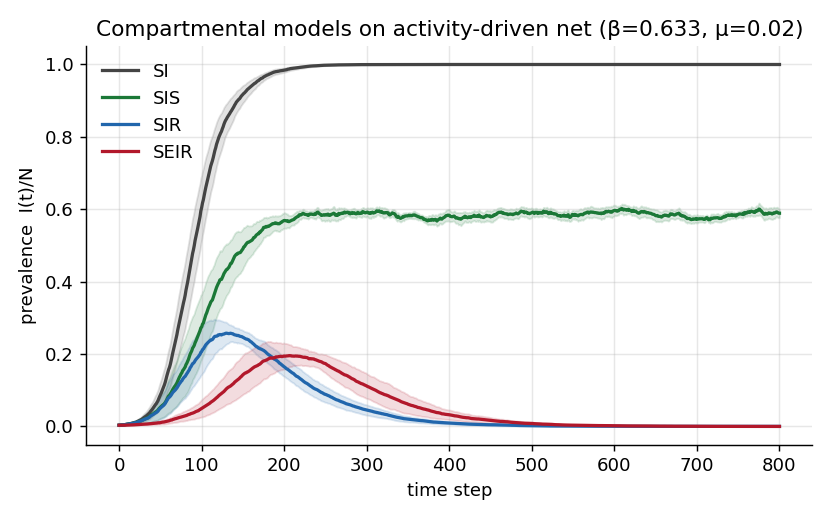
\includegraphics[width=\linewidth]{images/epidemics_fig1_models.png}\caption{Four models on the AD network}\end{subfigure}
\hfill
\begin{subfigure}{0.47\textwidth}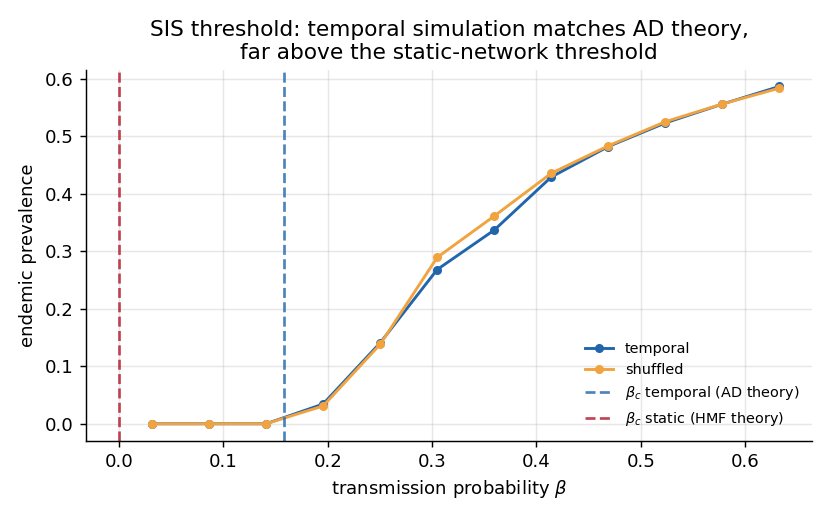
\includegraphics[width=\linewidth]{images/epidemics_fig2_threshold.png}\caption{SIS threshold vs.\ theory}\end{subfigure}
\\[4pt]
\begin{subfigure}{0.47\textwidth}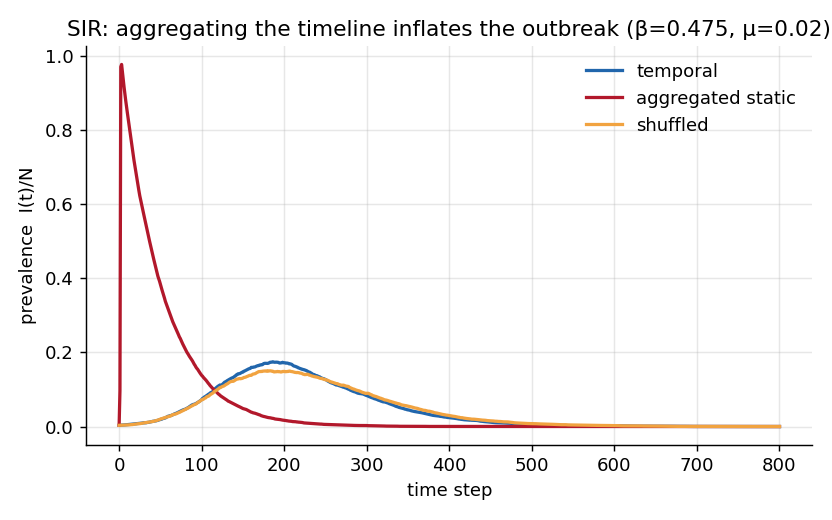
\includegraphics[width=\linewidth]{images/epidemics_fig3_temporal_vs_static.png}\caption{SIR: temporal vs.\ aggregated (AD)}\end{subfigure}
\hfill
\begin{subfigure}{0.47\textwidth}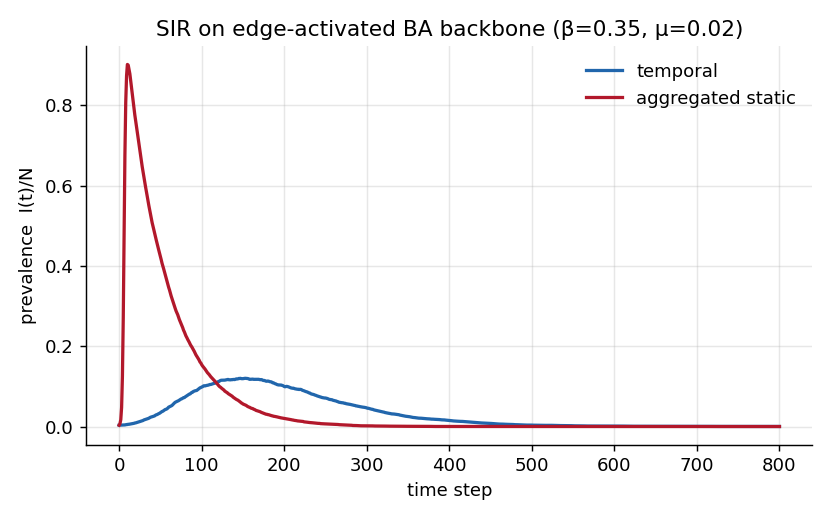
\includegraphics[width=\linewidth]{images/epidemics_fig4_backbone.png}\caption{SIR on the edge-activated BA backbone}\end{subfigure}
\caption{Epidemics on temporal networks. (a)~SI/SIS/SIR/SEIR prevalence on one
activity-driven network ($\beta=4\beta_c^{\mathrm{AD}}$); bands are $\pm1\sigma$
over realisations. (b)~SIS endemic prevalence vs.\ $\beta$: the temporal
simulation matches $\beta_c^{\mathrm{AD}}$ (dashed) and lies far above
$\beta_c^{\mathrm{HMF}}$; time-shuffled $\approx$ temporal. (c,d)~Aggregating the
timeline (red) inflates the SIR outbreak relative to the temporal dynamics (blue)
on both topologies.}
\label{fig:epi}
\end{figure}

Code and data (generators, engine, thresholds, edge lists) are in
\texttt{code/temporal\_epidemics/} and \texttt{data/temporal\_epidemics/}; see also
Holme \& Saram\"aki~\cite{holme2012temporal} for the temporal-network framework.

\newpage
